\section{TAN Trigonometric Tangent Function}

\subsection{Usage}

Computes the \verb|tan| function for its argument.  The general
syntax for its use is
\begin{verbatim}
  y = tan(x)
\end{verbatim}
where \verb|x| is an \verb|n|-dimensional array of numerical type.
Integer types are promoted to the \verb|double| type prior to
calculation of the \verb|tan| function.  Output \verb|y| is of the
same size and type as the input \verb|x|, (unless \verb|x| is an
integer, in which case \verb|y| is a \verb|double| type).  
\subsection{Function Internals}

Mathematically, the \verb|tan| function is defined for all real
valued arguments \verb|x| by the infinite summation
\[
  \tan x \equiv x + \frac{x^3}{3} + \frac{2x^5}{15} + \cdots,
\]
or alternately by the ratio
\[
  \tan x \equiv \frac{\sin x}{\cos x}
\]
For complex valued arguments \verb|z|, the tangent is computed via
\[
  \tan z \equiv \frac{\sin 2 \Re z + i \sinh 2 \Im z}
                     {\cos 2 \Re z + \cosh 2 \Im z}.
\]
\subsection{Example}

The following piece of code plots the real-valued \verb|tan(x)|
function over the interval \verb|[-1,1]|:
\begin{verbatim}
--> t = linspace(-1,1);
--> plot(t,tan(t))
\end{verbatim}


\centerline{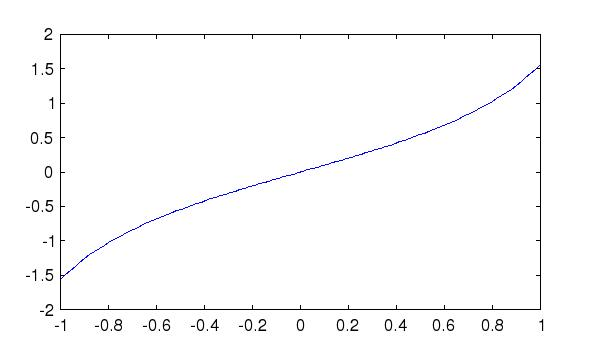
\includegraphics[width=8cm]{tanplot}}

